
\section{Question Answering}
\label{chap6:sec:qa}

In this section, we discuss the usage of post-training to question answering.
We focus on a novel review-based task called review reading comprehension (RRC).

\subsection{-- Motivation}
%\subsection{-- Review Reading Comprehension (RRC)}
\label{chap6:sec:rrc}

For online commerce, question-answering (QA) serves either as a standalone application of customer service or as a crucial component of a dialog system that answers user questions.
Many intelligent personal assistants (such as Amazon Alexa and Google Assistant) support online shopping by allowing the user to speak directly to the assistants. 
One major hindrance to this mode of shopping is that such systems have limited capability to answer user questions about products (or services), which are vital for customer decision making.
As such, an intelligent agent that can automatically answer customers' questions is very important for the success of online businesses.

Given the ever-changing environment of products and services, it is very hard, if not impossible, to pre-compile an up-to-date and reliable knowledge base to cover a wide assortment of questions that customers may ask, such as in factoid-based KB-QA \cite{xu2016question,fader2014open,kwok2001scaling,yin2015neural}.
As a compromise, many online businesses leverage community question-answering (CQA) \cite{mcauley2016addressing} to crowdsource answers from existing customers. However, the problem with this approach is that many questions are not answered, and if they are answered, the answers are delayed, which is not suitable for interactive QA.
We explore the usage of product reviews as a large knowledge pool of user experiences that can be exploited to answer users' questions. Although there are existing studies that have used information retrieval (IR) techniques \cite{mcauley2016addressing,yu2018aware} to find a whole review as the response to a user question, giving the whole review to the user is undesirable as it is quite time-consuming for the user to read it.

Inspired by the success of \underline{M}achine \underline{R}eading \underline{C}omphrenesions (MRC) \cite{rajpurkar2016squad,rajpurkar2018know}, we propose a novel task called \underline{R}eview \underline{R}eading \underline{C}omprehension (RRC) as following.

\textbf{Problem Definition}: Given a question $q=(q_1, \dots, q_m)$ from a customer (or user) about a product and a review $d=(d_1, \dots, d_n)$ for that product containing the information to answer $q$, find a sequence of tokens (a text span) $a=(d_s, \dots, d_e)$ in $d$ that answers $q$ correctly, where $1 \le s \le n$, $1\le e \le n$, and $s\le e$.

\begin{table}
    \centering
    \scalebox{0.87}{
        \begin{tabular}{|l|}
            \hline
            {\bf Questions}\\
            \hline
            Q1: Does it have an internal hard drive ?\\
            Q2: How large is the internal hard drive ?\\
            Q3: is the capacity of the internal hard drive OK ?\\
            \hline
            {\bf Review}\\
            Excellent value and a must buy for someone \\
            looking for a Macbook . You ca n't get any \\
            better than this price and it \textbf{come with}\textsubscript{A1} an\\
            internal disk drive . All the newer MacBooks\\
            do not . Plus you get \textbf{500GB}\textsubscript{A2} which is also a\\
            \textbf{great}\textsubscript{A3} feature . Also , the resale value on \\
            this will keep . I highly recommend you get one \\
            before they are gone .\\
            \hline
        \end{tabular}
    }
    %\caption{Review reading comprehension: we show 3 questions and their corresponding answer spans from a review.}
    \caption{Review reading comprehension}
    \label{chap6:tbl:example}
\end{table}

A sample \emph{laptop} review is shown in \ref{chap6:tbl:example}. 
We can see that customers may not only ask factoid questions such as the specs about some aspects of the laptop as in the first and second questions but also subjective or opinion questions about some aspects (capacity of the hard drive), as in the third question.
RRC poses some \textit{domain challenges} compared to the traditional MRC on Wikipedia, such as the need for rich product knowledge, informal text, and fine-grained opinions (there is almost no subjective content in Wikipedia articles). Research also shows that yes/no questions are very frequent for products with complicated specifications \cite{mcauley2016addressing,Xu2018pro}.

To my knowledge, there is no existing work on RRC. 
We first build a dataset called ReviewRC, using reviews from SemEval 2016 Task 5\footnote{\url{http://alt.qcri.org/semeval2016/task5/}. We choose these review datasets to align RRC with existing research on sentiment analysis.}, which is a popular dataset for aspect-based sentiment analysis (ABSA) \cite{hu2004mining} in the domains of \emph{laptop} and \emph{restaurant}.
We detail ReviewRC in Chapter \ref{chap6:sec:exp}.
Given the wide spectrum of domains (types of products or services) in online businesses and the prohibitive cost of annotation, ReviewRC can only be considered to have a limited number of annotated examples for supervised training, which still leaves the domain challenges partially unresolved.

To simplify the writing, we refer MRC as a general-purpose RC task on formal text (non-review) and RRC as an end-task specifically focused on reviews.), where the former enhances domain-awareness and the latter strengthens MRC task-awareness.
Although BERT gains great success on SQuAD, this success is based on the huge amount of training examples of SQuAD (100,000+).
This amount is large enough to ameliorate the flaws of BERT that has almost no questions on the left side and no textual span predictions based on both the question and the document on the right side.
However, a small amount of fine-tuning examples is not sufficient to turn BERT to be more task-aware.

\textbf{Related Works}

Many datasets have been created for MRC from formally written and objective texts. 
For example, some datasets are from Wikipedia
(SQuAD \cite{rajpurkar2016squad,rajpurkar2018know}, WikiHop \cite{welbl2018constructing}, DRCD \cite{shao2018drcd}, QuAC \cite{choi2018quac}, HotpotQA \cite{yang2018hotpotqa}). 
Also, CoQA \cite{reddy2018coqa} is built from multiple sources, such as Wikipedia, Reddit, News, Mid/High School Exams, Literature, etc.
To the best of our knowledge, MRC has not been used on primarily subjective reviews. As such, we created a review-based MRC dataset called ReviewRC.
Answers from ReviewRC are extractive (similar to SQuAD \cite{rajpurkar2016squad,rajpurkar2018know}) rather than abstractive (or generative) (such as in MS MARCO \cite{nguyen2016ms} and CoQA \cite{reddy2018coqa}).
This is crucial because online businesses are typically cost-sensitive and extractive answers written by humans can avoid generating incorrect answers beyond the contents in reviews by an AI agent.

Community QA (CQA) is widely adopted by online businesses \cite{mcauley2016addressing} to help users.
However, since it solely relies on humans to give answers, it often takes a long time to get a question answered or even not answered at all as we discussed in the introduction.
Although there exists researches that align reviews to questions as an information retrieval task \cite{mcauley2016addressing,yu2018aware}, giving a whole review to the user to read is time-consuming and not suitable for customer service settings that require interactive responses.

Knowledge bases (KBs) (such as Freebase \cite{dong2015question,xu2016question,yao2014information} or DBpedia \cite{lopez2010scaling,unger2012template}) have been used for question answering \cite{yu2018aware}.
However, the ever-changing nature of online businesses, where new products and services appear constantly, makes it prohibitive to build a high-quality KB to cover all new products and services.

Reviews also serve as a rich resource for sentiment analysis \cite{pang2002thumbs,hu2004mining,liu2012sentiment,liu2015sentiment}.
Although document-level (review) sentiment classification may be considered as a solved problem (given ratings are largely available), aspect-based sentiment analysis (ABSA) is still an open challenge, where alleviating the cost of the human annotation is also a major issue.
ABSA aims to turn unstructured reviews into structured fine-grained aspects (such as the ``battery'' of a laptop) and their associated opinions (e.g., ``good battery'' is \emph{positive} about the aspect battery).
Two important tasks in ABSA are aspect extraction (AE) and aspect sentiment classification (ASC) \cite{hu2004mining}, where the former aims to extract aspects (e.g., ``battery'') and the latter targets to identify the polarity for a given aspect (e.g., \emph{positive} for \emph{battery}).
Recently, supervised deep learning models dominate both tasks \cite{wang2016recursive,wang2017coupled,xu_acl2018,tang2016aspect,he2018exploiting} and many of these models use handcrafted features, lexicons, and complicated neural network architectures to remedy the insufficient training examples from both tasks.
Although these approaches may achieve better performances by manually injecting human knowledge into the model, human baby-sat models may not be intelligent enough\footnote{\url{http://www.incompleteideas.net/IncIdeas/BitterLesson.html}} and automated representation learning from review corpora is always preferred \cite{xu_acl2018,he2018exploiting}.
We push forward this trend with the recent advance in pre-trained language models from deep learning~\cite{peters2018deep,howard2018universal,devlin2018bert,radford2018improving,radford2018lang}. 
Although it is practical to train domain word embeddings from scratch on large-scale review corpora \cite{xu_acl2018}, it is impractical to train language models from scratch with limited computational resources.
As such, we show that it is practical to adopt language models pre-trained from formal texts to domain reviews.

RRC may suffer from the prohibitive cost of annotating large-scale training data covering a wide range of domains. 
And BERT severely lacks two kinds of prior knowledge: (1) large-scale domain knowledge (e.g., about a specific product category), and (2) task-awareness knowledge (MRC/RRC in this case).
We detail the technique of jointly incorporating these two types of knowledge as a post-training stage in Chapter \ref{chap4:context}.

\textbf{Results}

As there are no existing datasets for RRC and
to be consistent with existing research on sentiment analysis, we adopt the \textit{laptop} and \textit{restaurant} reviews of SemEval 2016 Task 5 as the source to create datasets for RRC.
We do not use SemEval 2014 Task 4 or SemEval 2015 Task 12 because these datasets do not come with the review(document)-level XML tags to recover whole reviews from review sentences.~We keep the split of training and testing of the SemEval 2016 Task 5 datasets and annotate multiple QAs for each review following the way of constructing QAs for the SQuAD 1.1 datasets \cite{rajpurkar2016squad}.

To make sure our questions are close to real-world questions, 2 annotators are first exposed to 400 QAs from CQA (under the laptop category in Amazon.com or popular restaurants in Yelp.com) to get familiar with real questions.
Then they are asked to read reviews and independently label textual spans and ask corresponding questions when they feel the textual spans contain valuable information that customers may care about.
The textual spans are labeled to be as concise as possible but still human-readable.
Note that the annotations for sentiment analysis tasks are not exposed to annotators to avoid biased annotation on RRC.
Since it is unlikely that the two annotators can label the same QAs (the same questions with the same answer spans), they further mutually check each other's annotations and disagreements are discussed until agreements are reached.~Annotators are encouraged to label as many questions as possible from testing reviews to get more test examples. A training review is encouraged to have 2 questions (training examples) on average to have good coverage of reviews.

The annotated data is in the format of SQuAD 1.1 \cite{rajpurkar2016squad} to ensure compatibility with existing implementations of MRC models. The statistics of the RRC dataset (ReviewRC) are shown in \ref{chap6:tbl:rrc}. 
Since SemEval datasets do not come with a validation set, we further split 20\% of reviews from the training set for validation.

\begin{table}[H]
    \centering
    \scalebox{0.7}{
        \begin{tabular}{c||c|c}
        \hline
        {\bf Dataset} &{\bf Num. of Questions } &{\bf Num. of Reviews }  \\
        \hline
        Laptop Training & 1015 & 443 \\
        Laptop Testing & 351 & 79 \\
        \hline
        Restaurant Training & 799 & 347 \\
        Restaurant Testing & 431 & 90 \\
        \hline
        \end{tabular}
    }
    %\caption{Statistics of the ReviewRC Dataset. Reviews with no questions are ignored.}
    \caption{Statistics of ReviewRC Dataset}
\label{chap6:tbl:rrc}
\end{table}


\textbf{Compared Methods}

As BERT outperforms existing open-source MRC baselines by a large margin, we do not intend to exhaust existing implementations but focus on variants of BERT introduced in this paper.

\textbf{DrQA} is a baseline from the document reader\footnote{https://github.com/facebookresearch/DrQA} of DrQA \cite{chen2017reading}.~We adopt this baseline because of its simple implementation for reproducibility.~We run the document reader with random initialization and train it directly on ReviewRC.
We use all default hyper-parameter settings for this baseline except the number of epochs, which is set as 60 for better convergence.

\textbf{DrQA+MRC} is derived from the above baseline with official pre-trained weights on SQuAD.
We fine-tune document reader with ReviewRC. We expand the vocabulary of the embedding layer from the pre-trained model on ReviewRC since reviews may have words that are rare in Wikipedia and keep other hyper-parameters as their defaults.

For AE and ASC, we summarize the scores of the state-of-the-arts on SemEval (based the best of our knowledge) for brevity.\\

Lastly, we have the following BERT variants.\\
\textbf{BERT} is the vanilla BERT fine-tuned on all 3 end tasks. We use this baseline to show that BERT's pre-trained weights alone have limited performance gains on review-based tasks.\\
\textbf{BERT-DK} post-trains BERT's weights only on domain knowledge (reviews) and fine-tunes on the 3 end tasks. We use BERT-DK and the following BERT-MRC.\\
\textbf{BERT-MRC} post-trains BERT's weights on SQuAD 1.1 and then fine-tunes on the 3 end tasks.\\
\textbf{BERT-PT} (proposed method) post-trains BERT's weights using the joint post-training algorithm in Section \ref{chap4:sec:post-training} and then fine-tunes on the 3 end tasks.

\textbf{Evaluation Metrics and Model Selection}

To be consistent with existing research on MRC,
we use the same evaluation script from SQuAD 1.1 \cite{rajpurkar2016squad} for RRC, which reports Exact Match (EM) and F1 scores.
EM requires the answers to have an exact string match with human-annotated answer spans.
F1 score is the averaged F1 scores of individual answers, which is typically higher than EM and is the major metric.
Each F1 score is the (harmonic) mean of individual precisions and recalls. It is computed based on the number of overlapped words between the predicted answer and human-annotated answers.

We set the maximum number of epochs to 4 for BERT variants, though most runs converge just within 2 epochs.
Results are reported as averages of \textbf{9} runs (9 different random seeds for random batch generation).\footnote{We notice that adopting 5 runs used by existing researches still has a high variance for a fair comparison.} 

\textbf{Result Analysis}

\begin{table}[H]
    \centering
    \scalebox{0.7}{
        \begin{tabular}{l||c c|c c}
        \hline
        {\bf Domain} & {\bf Laptop} & & {\bf Rest.} & \\
        \hline
        {\bf Methods} & {\bf EM } &{\bf F1 } & {\bf EM } & {\bf F1 } \\
        \hline
        DrQA\cite{chen2017reading} & 38.26 & 50.99 & 49.52 & 63.73 \\
        DrQA+MRC\cite{chen2017reading} & 40.43 & 58.16 & 52.39 & 67.77 \\
        \hline
        BERT & 39.54 & 54.72 & 44.39 & 58.76 \\
        BERT-DK & 42.67 & 57.56 & 48.93 & 62.81 \\
        BERT-MRC &  47.01 & 63.87 & 54.78 & 68.84 \\
        BERT-PT & 48.05 & \textbf{64.51} & 59.22 & \textbf{73.08} \\
        \hline
        \end{tabular}
    }
    \caption{RRC in EM (Exact Match) and F1.}
\label{chap6:tbl:result_rc}
\vspace{-3mm}
\end{table}


The results of RRC are shown in \ref{chap6:tbl:result_rc}. 
We observed that the proposed joint post-training (BERT-PT) has the best performance on all tasks in all domains, which show the benefits of having two types of knowledge.
To our surprise, we found that the vanilla pre-trained weights of BERT do not work well for review-based tasks, although it achieves state-of-the-art results on many other NLP tasks \cite{devlin2018bert}.
This justifies the need to adapt BERT to review-based tasks.
We noticed that the roles of domain knowledge and task knowledge vary for different tasks and domains.
For RRC, we found that the performance gain of BERT-PT mostly comes from task-awareness (MRC) post-training (as indicated by BERT-MRC).
The domain knowledge helps more for restaurant than for laptop.
We suspect the reason is that certain types of knowledge (such as specifications) of laptop are already present in Wikipedia, whereas Wikipedia has little knowledge about restaurant.
We further investigated the examples improved by BERT-MRC and found that the boundaries of spans (especially short spans) were greatly improved. 

The errors on RRC mainly come from boundaries of spans that are not concise enough and incorrect location of spans that may have certain nearby words related to the question. 
We believe precisely understanding user's experience is challenging from only domain post-training given limited help from the RRC data and no help from the Wikipedia data.

\section{Dialog System}
\label{chap6:sec:dialog}

Given the recent popularity of research in dialog system, I further discuss the usage of lifelong representation learning for conversational AI.
I mainly focus on two tasks: one is the extension of RRC discussed in the previous section; the other is a novel task called conversational recommendation that aims to learn dynamic graph reasoning.

\subsection{-- Review Conversational Reading Comprehension (RCRC)}
\label{chap6:sec:rcrc}

%Inspired by conversational reading comprehension (CRC), this work studies a novel task of leveraging reviews as a source to build an agent that can answer multi-turn questions from potential consumers of online businesses. We first build a review CRC dataset and then propose a novel task-aware pre-tuning step running between language model (e.g., BERT) pre-training and domain-specific fine-tuning.~The proposed pre-tuning requires no data annotation, but can greatly enhance the performance on our end task. Experimental results show that the proposed approach is highly effective and has competitive performance as the supervised approach.

Seeking information to assess whether a product or service suits one's needs is an important activity in consumer decision making.
One major hindrance for online businesses is that the consumers often have difficulty to get answers to their questions.
With the ever-changing environment, it is very hard, if not impossible, for businesses to pre-compile an up-to-date knowledge base to answer user questions as in KB-QA \cite{kwok2001scaling,fader2014open,yin2015neural,xu2016question}.
Although community question-answering (CQA) helps~\cite{mcauley2016addressing}, one has to be lucky to get an existing customer to answer a question quickly. There is work on retrieving whole reviews relevant to a question~\cite{mcauley2016addressing,yu2018aware}, but it is not ideal for the user to read the whole reviews to fish for answers.

\begin{table}
    \centering
    \scalebox{0.75}{
        \begin{tabular}{l}
            \hline
            {\bf A Laptop Review:}\\
            \hline
            I purchased my Macbook Pro Retina from my school since I \\
            had a student discount , but I would gladly purchase it from \\
            Amazon for full price again if I had too . The Retina is \textcolor{purple}{\textbf{great}} \\
            , its \textcolor{red}{\textbf{amazingly fast}} when it boots up because of the \textcolor{orange}{\textbf{SSD}}\\
            \textcolor{orange}{\textbf{storage}} and the clarity of the screen is \textcolor{blue}{\textbf{amazing}} as well...\\
            \hline
            {\bf Turns of Questions from a Customer:}\\
            \hline
            \textcolor{purple}{$q_1$: how is retina display ?}\\
            \textcolor{red}{$q_2$: speed of booting up ?}\\
            \textcolor{orange}{$q_3$: why ?}\\
            \textcolor{cyan}{$q_4$: what 's the capacity of that ? (NO ANSWER)}\\
            \textcolor{blue}{$q_5$: is the screen clear ?}\\
            \hline
        \end{tabular}
    }
    \label{chap6:tbl:crc_example}
    \caption{Review conversational reading comprehension (RCRC)}   
    %\caption{Review conversational reading comprehension (RCRC) (best viewed in colors): a dialog with 5 turns of customers' questions and answer spans from a review.}
\end{table}

    
Inspired by conversational reading comprehension (CRC) \cite{reddy2018coqa,choi2018quac,xu-etal-2019-bert}, we explore the possibility of turning reviews into a valuable source of knowledge of real-world experiences and using it to answer customer or user multi-turn questions.~We call this \textit{\underline{R}eview \underline{C}onversational \underline{R}eading \underline{C}omprehension} (RCRC).
The conversational setting enables the user to go into details via more specific questions and to simplify their questions by either omitting or co-referencing information in the previous context.
As shown in \ref{chap6:tbl:crc_example}, 
the user first has an \textit{opinion} question about ``retina display'' (an \textit{aspect}) of a laptop.~Then he/she carries (or omits) the question type \textit{opinion} from the first question to the second question about another \textit{aspect} ``boot-up speed''.
Later, he/she carries the \textit{aspect} of the second question, but changes the question type to \textit{opinion reason} and then co-references the \textit{aspect} ``SSD'' from the third answer and asks for the capacity (a \textit{sub-aspect}) of ``SSD''.
Unfortunately, there is no answer in this review. 
Finally, the customer asks another \textit{aspect} as in the fifth question. RCRC is defined as follows.

\noindent\textbf{RCRC Definition}: Given a review that consists of a sequence of $n$ tokens $d=(d_1, \dots, d_n)$, a history of past $k-1$ questions and answers as the context $C=(q_1, a_1, q_2, a_2, \dots, q_{k-1}, a_{k-1})$ and the current question $q_k$, find a sequence of tokens (a textual span) $a=(d_s, \dots, d_e)$ in $d$ that answers $q_k$ based on $C$, where $1 \le s \le n$, $s\le e \le n$, and $s\le e$, or return \textit{NO ANSWER} ($s, e=0$) if the review does not contain the answer for $q_k$.

Note that although RCRC focuses on one review, it can potentially be deployed on the setting of multiple reviews (e.g., all reviews for a product), where the context $C$ may contain answers from different reviews.
To the best of our knowledge, there are no existing review datasets for RCRC. We first build a dataset called $(\text{RC})_2$ based on laptop and restaurant reviews from SemEval 2016 Task 5.\footnote{\url{http://alt.qcri.org/semeval2016/task5/} We choose this dataset to better align with existing research in sentiment analysis.} 

Given the wide spectrum of domains in online businesses and the prohibitive cost of annotation, $(\text{RC})_2$ has limited training data,
as in many other tasks of sentiment analysis.

As a result, the challenge is how to effectively improve the performance of RCRC.
We adopt BERT \cite{devlin2018bert} as our base model since it can be either a feature encoder or a standalone model that achieves good performance on CRC \cite{reddy2018coqa}.
BERT bears with task-agnostic features, which require task-specific architecture and many supervised training examples to train(fine-tune) on an end task.
As $(\text{RC})_2$ has limited training data, 
we propose a novel task-aware \textit{pre-tuning} to further bridge the gap between BERT pre-training and RCRC task-awareness, as discussed in Chapter \ref{chap4:context}.
Pre-tuning requires no annotation of CRC (or RCRC) data but just QA pairs (from CQA) and reviews that are largely available online.
The data are general and can potentially be used in other machine reading comprehension tasks.
Experimental results show that the proposed approach achieves competitive performance even compared with the supervised approach using a large-scale annotated dataset.


\textbf{Datasets}

We adopt SemEval 2016 Task 5
as the review source for RCRC (to be consistent with research in sentiment analysis), which contains two domains \textit{laptop} and \textit{restaurant}.
We kept the split of training and testing and annotated dialogs on each review.
The annotation guideline can be found in supplemental material\footnote{The annotated data is in the format of CoQA \cite{reddy2018coqa} to help future research. But we do not focus on generative annotation as in CoQA because businesses are sensitive to errors of generative models}.
To ensure questions are real-world questions, annotators are first asked to read hundreds of community questions and answers (CQA) from real customers.
The statistics of the annotated $(\text{RC})_2$ dataset is shown in \ref{chap6:tbl:rcrc}.
We use 20\% of the training reviews as the validation set for each domain.

\begin{table}
    \centering
    \scalebox{0.8}{
        \begin{tabular}{c||c|c}
        \hline
        Training &{\bf Laptop } &{\bf Restaurant} \\
        \hline
        \# of reviews & 445 & 350\\
        \# of dialogs & 506 & 382\\
        \# of dialog /w 3+ turns & 375 & 315\\
        \# of questions & 1679 & 1486\\
        \% of no answers & 24.3\%& 24.2\%\\
        \hline
        Testing &{\bf Laptop } &{\bf Restaurant} \\
        \hline
        \# of reviews & 79 & 90 \\
        \# of dialog & 170 & 160 \\
        \# of dialog /w 3+ turns & 148 & 135\\
        \# of questions & 804 & 803 \\
        \% of no answers & 26.6\% & 28.0\% \\
        \hline
        \end{tabular}
    }
\label{chap6:tbl:rcrc}
\caption{Statistics of $(\text{RC})_2$ Datasets.}
\vspace{-5mm}
\end{table}

For the proposed pre-tuning, we collect QA pairs and reviews for these two domains.
For \emph{laptop}, we collect the reviews from \cite{he2016ups} and QA pairs from \cite{Xu2018pro} both under the laptop category of Amazon.com. We exclude products in the test data of $(\text{RC})_2$.
This gives us 113,728 laptop reviews and 19,104 QA pairs. 
For \emph{restaurant}, we crawl reviews and all QA pairs from the top 60 restaurants in each U.S. city from Yelp.com.
This ends with 197,333 restaurant reviews and 49,587 QA pairs. Based on the number of QAs, Algorithm 1 is run $k=10$ times for laptop and $k=5$ times for restaurant.

To compare with the performance of a fully-supervised approach,~we leverage the CoQA dataset with 7,199 documents (covering domains in Children’s Story, Mid/High School Literature, News, Wikipedia, etc.) and 108,647 turns of question/answer span annotated via crowdsourcing.

\textbf{Compared Methods}

We compare the following methods: \\
\textbf{DrQA} is a CRC baseline coming with the CoQA dataset\footnote{https://github.com/stanfordnlp/coqa-baselines}. \\
\textbf{DrQA+CoQA} is the above baseline pre-tuned on the CoQA dataset and then fine-tuned on $(\text{RC})_2$ to show that even DrQA pre-trained on CoQA is sub-optimal.\\
\textbf{BERT}\footnote{We choose $\text{BERT}_{\text{BASE}}$ as we cannot fit $\text{BERT}_{\text{LARGE}}$ into the memory.} is the pre-trained BERT weights directly fine-tuned on $(\text{RC})_2$ for ablation study on the effectiveness of pre-tuning.\\
\textbf{BERT+review} first tunes BERT on domain reviews using the same objectives as BERT pre-training and then fine-tunes on $(\text{RC})_2$. We use this baseline to show that a simple domain-adaptation of BERT is not sufficient.\\
\textbf{BERT+CoQA} first fine-tunes BERT on the supervised CoQA data and then fine-tunes on $(\text{RC})_2$. We use this method to show that our pre-tuning is still very competitive even compared with using this large-scale supervised data.\\
\textbf{BERT+Pre-tuning} is the proposed approach.

\textbf{Hyper-parameters and Evaluation}

We set the maximum length of BERT to 256 with the maximum length of context+question to 96 ($h_\text{max}=9$ for Algorithm \ref{chap4:alg:pre-tuning}) and the batch size to 16.
We perform pre-tuning for 10k steps. 
CoQA fine-tuning converges in 2 epochs.
Fine-tune RCRC is performed for 4 epochs and most runs converged within \textbf{3} epochs.
We search the maximum number of turns in context $C$ for RCRC fine-tuning using the validation set, which ends with 6 turns for laptop and 5 turns for restaurant.
Results are reported as averages of 3 runs.
To be consistent, we leverage the same evaluation script as CoQA, which reports 
turn-level Exact Match (EM) and F1 scores for all turns in all dialogs.

\begin{table}
    \centering
    \scalebox{0.7}{
        \begin{tabular}{l||c c|c c}
        \hline
        {\bf Domain} & {\bf Laptop} & & {\bf Rest.} & \\
        \hline
        {\bf Methods} & {\bf EM } &{\bf F1 } & {\bf EM } & {\bf F1 } \\
        \hline
        DrQA & 28.5 & 36.6 & 41.6 & 50.3 \\
        DrQA+CoQA(supervised) & 40.4 & 51.4 & 47.7 & 58.5 \\
        \hline
        \hline
        BERT & 38.57 & 48.67 & 46.87 & 55.07 \\
        BERT+review & 34.53 & 43.83 & 47.23 & 53.7 \\
        BERT+CoQA(supervised) & 47.1 & 58.9 & 56.57 & 67.97 \\
        BERT+Pre-tuning & 46.0 & 57.23 & 54.57 & 64.43 \\
        \hline
        \end{tabular}
    }
    \caption{RCRC on EM (Exact Match) and F1.}
\label{chap6:tbl:result_rcrc}
\vspace{-7mm}
\end{table}

\textbf{Result Analysis}

As shown in \ref{chap6:tbl:result_rcrc}, 
BERT+Pre-tuning has significant performance gains over BERT fine-tuned directly on $(\text{RC})_2$ by \textbf{9\%}.
BERT is overall better than DrQA.
But directly using review documents to adapt BERT does not yield better results as in BERT+review.
We suspect the task of RCRC still requires a certain degree of general language understanding on the question side and BERT+review also has the effect of (catastrophic) forgetting \cite{kirkpatrick2017overcoming} on such representation.
Further, large-scale annotated CoQA data can boost the performance for both DrQA and BERT.
However, our pre-tuning approach still has competitive performance and it requires no annotation at all.
We examine the errors of BERT+Pre-tuning and realize that both locations of span and span boundaries tend to have errors, indicating a significant room for improvement.

\subsection{-- Memory-grounded Conversational Recommendation}
\label{chap6:sec:mgcr}

Conversational recommendation aims to collect users' up-to-date preferences through dialog, instead of relying only on preferences learned offline.
However, most existing systems make an unnatural assumption that users' preferences can only be collected offline or online, and neglect the fact that the knowledge about a user is dynamic and cumulative.
To this end, we propose a novel concept called \textit{user memory graph}, which aims to maintain the knowledge about a user in a structured form for interpretability.
Each turn of the dialog is grounded onto this user memory graph for the reasoning of dialog policy, and more importantly, further accumulation of user knowledge.

\textbf{Motivation}

Traditional recommender systems (such as the collaborative filtering (CF) system) often aim to learn the static correlations between users' preferences and associated items' attributes.
While it is a powerful approach that can leverage the vast offline user preferences data for effective recommendations, such a system is challenged when operating in the dynamic world, in which new users and items unseen during training frequently appear (so-called cold-start problems).
More importantly, static systems fail to capture users' preferences that may change from time to time.

%\begin{figure}
%\centering    
%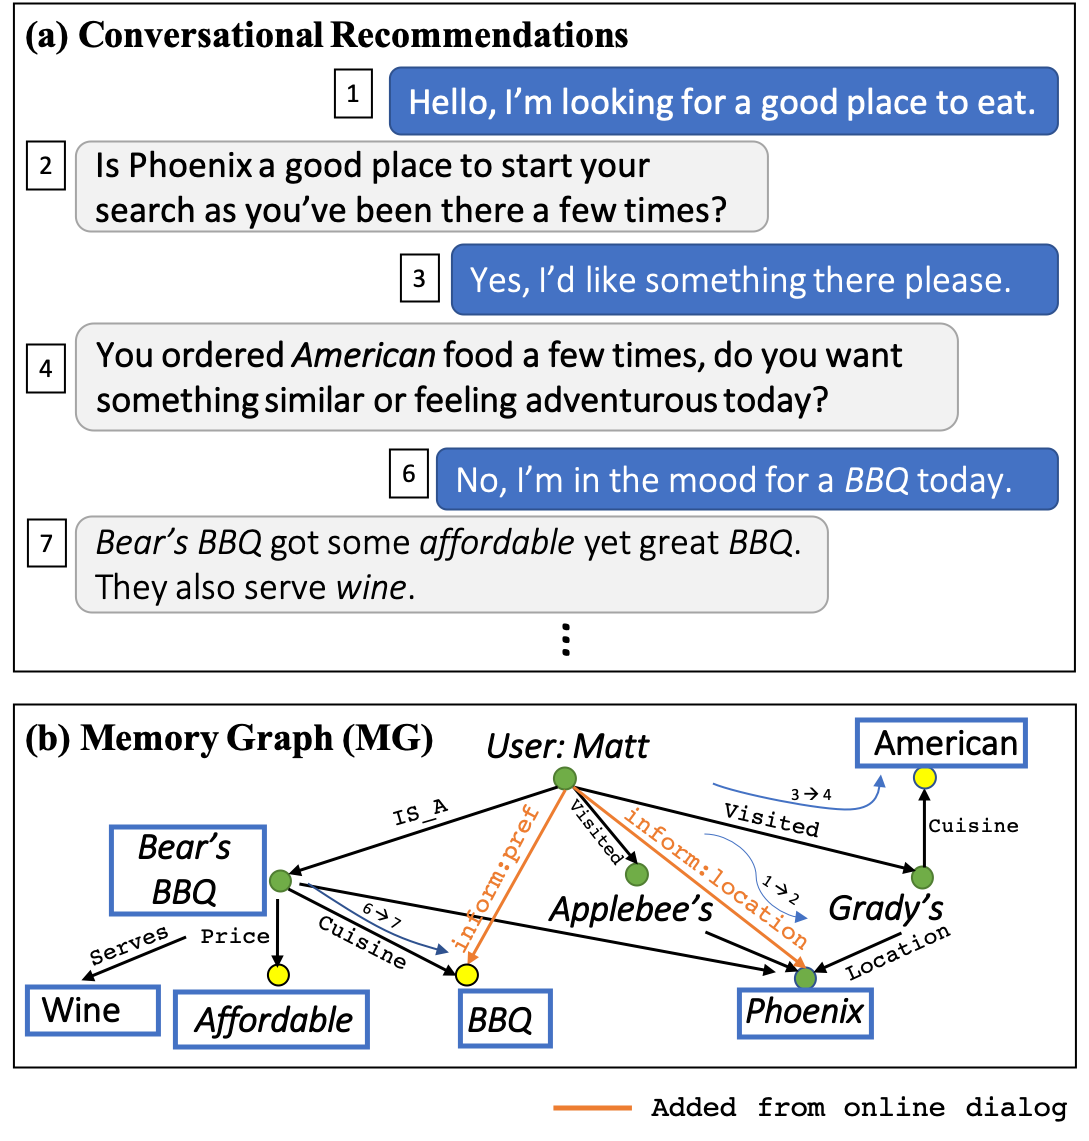
\includegraphics[width=0.9\columnwidth]{fig/acl19_teaser.png}
    %\caption{A conceptual illustration of \textbf{Memory-grounded conversational recommendation}. (1) Conversational recommendation allows users to express preferences and requirements through dialogs. (2) Our \textit{MGConvRex} corpus is grounded on the memory graph (MG), which represents user's past preferences as well as newly added preferences.}
    %\caption{Conceptual illustration of %Memory-grounded conversational recommendation}
%\label{fig:dialog}
%\vspace{-3mm}
%\end{figure}

Conversational recommendation systems \cite{li2018towards} are recently introduced to mitigate some of these challenges by tracking users' up-to-date preferences through dialogs.
Most of the previous works focus on extending the conventional task-oriented dialog literature with a recommender system, which allows the conversational system to update user preferences online by asking relevant questions (called ``System Ask User Respond (SAUR)'' for the current dialog.

In summary, existing systems either favor a static offline recommendation over existing users or items or obtain short-term online updates on users' preferences via dialogs.
However, they unnaturally contrast offline with online preference learning and neglect the fact that the knowledge about a user is \textit{cumulative} in nature.
An intelligent system should be able to dynamically maintain and utilize knowledge about a user collected so far for recommendations.

To this end, we first introduce a novel concept called \textit{user memory graph} to represent dynamic knowledge about users and associated items in a structured graph (e.g., previous offline history of items visited/recommended, user preferences newly obtained through dialogs, etc.), allowing for easy and holistic reasoning for recommendations.
We then propose a new conversational recommendation system grounded onto this graph, conceptually defined more formally as follows:

\noindent\textbf{Memory-grounded Conversational Recommendation}:
Given the history of previous items $\mathcal{H}$ (interacted or visited, etc.), candidate items $\mathcal{C}$ for recommendation, and their attributes (values), 
an agent first (1) constructs a user memory graph $\mathcal{G} = \{(e, r, e')\vert e, e' \in \mathcal{E}, r \in \mathcal{R} \}$ for user $e_u$; 
then (2) for each turn $d \in D$ of a dialog, the agent updates $\mathcal{G}$ with tuples of preference $\mathcal{G}' \gets \mathcal{G} \cup \{(e_u, r_1, e_1), \dots\}$ ;
(3) performs reasoning over $\mathcal{G}'$ to yield a dialog policy $\pi$ that
either (i) performs more rounds of interaction by asking for more preference, 
or (ii) predicts optimal (or ground truth) items for recommendations $\mathcal{T} \subset \mathcal{C}$.

\textbf{Related Work}

\noindent \textbf{Conversational Recommendation}:
Much existing research on conversational recommendation focus on combining a recommender system with a dialog state tracking system, through the ``System Ask User Respond (SAUR)'' paradigm.
Once enough user preference is collected, such systems often make personalized recommendations to the user.
For instance, \cite{li2018towards} proposes to mitigate cold-start users by learning users' preferences during conversations and by linking the learned preferences to existing similar users in a traditional recommender system.

\cite{sun2018conversational,kang2019recommendation} propose a reinforcement learning (RL) setting for a conversational recommendation system, where the dialog policy is learned with multiple policies and recommendation signals.

\cite{zhang2018towards} leverages reviews to mimic online conversations to update an existing user's preference and re-rank items.

\noindent \textbf{Task-oriented Dialogue Systems} are widely studied with multiple popular benchmark datasets \cite{dstc2, woz, multiwoz, multiwoz2.1,sgd-dst}.
Most of the state-of-the-art approaches \cite{trade,bert-dst-alexa,bert-dst-cmu} focus on improving dialog state tracking with span-based pointer networks, which predicts information essential in completing a specified task (e.g., hotel booking, etc.)

Note that while conversational recommendation systems bears similarity to task-oriented dialog systems, the key difference is that conversational recommendation aims to collect user's fine-grained soft preferences or sentiments, and utilize them collectively for ranking of items or asking better questions (policy selection), instead of collecting hard constraints (e.g., number of people, time and location) to filter a database and locate a record. 

\noindent \textbf{Graph Reasoning}:
Graph network \cite{scarselli2008graph,duvenaud2015convolutional,defferrard2016convolutional,kipf2016semi} is a type of neural networks proposed to operate on graph structures. 
Several extensions to the original GCN have been proposed \cite{li2015gated,pham2017column}.
R-GCNs \cite{schlichtkrull2018modeling} can be applied to large-scale and highly multi-relational data.
Many applications of GNNs include \cite{Xian2019ReinforcementKG}, which introduces graph-based reasoning for an offline recommendation system.
A few works have recently been proposed to allow graph reasoning in dialog systems.
\cite{Moon+19a, Moon+19b} propose a new corpus to learn knowledge graph paths that connect dialog turns.
\cite{tuan-etal-2019-dykgchat} introduces a knowledge-grounded dialog generation task given a knowledge graph that is dynamically updated.
However, these workes often focus on response generation and do not address the conversational recommendation task.


\textbf{Definition of Dialog Acts, SLots and Values}

\label{chap6:sec:form}
One key step to enable a dialog being grounded and maintained on a user memory graph is to first define the semantic space of dialog acts, items, their slots and values (we borrow these terms from task-oriented dialog system, which refer to items' attributes) for utterances from both the user and agent.
As a result, agents can turn unstructured utterances into structured data for user memory graph maintenance, integration and potentially future explainable reasoning for policy.
In this section, we first introduce the dialog acts for recommendation and then introduce slots and values specifically defined for the recommendation in a restaurant domain.

\textbf{Dialog Acts}
\label{chap6:sec:dialog_act}

The goal of designing dialog acts $\mathcal{A}$ is to formalize the intentions from both the user and agent sides. 
\ref{chap6:tbl:dialog_act} demonstrates the dialog acts for both the user and the agent.
From the agent's perspective, 
note that although existing conversational recommendation\cite{sun2018conversational,li2018towards,zhang2018towards} assumes a passive user interacts with the system and propose a System Ask – User Respond (SAUR) paradigm, we further allow the user to actively participate in the recommendation by allowing User Ask - System Respond (UASR) paradigm. In our dialog act, \textit{Open question}, \textit{Yes/no question} and \textit{Inform} can be used by a user to actively participate in the conversation. The dataset we created from crowd workers also indicates that human likes to use these active dialog acts in the context of conversational recommendation.


\begin{table}
    \centering
    \scalebox{0.65}{
        \begin{tabular}{l|l l}
        \hline
        \textbf{Dialog Act $a$} & \textbf{Description} & \textbf{Examples} \\
        \hline
        \textbf{User-side} & & \\
        \hline
        Greeting & Greeting to the agent & I'd like to find a place to eat. \\
        Inform & Actively inform the agent your preference & I'd like to find a \textit{thai} restaurant . \\
        Answer & Answer to a question from the agent & I prefer \textit{thai} food. \\
        Reply & Reply to a recommendation & I'll give it a try.\\
        Open question & Actively ask an open question about a recommended item. & What kind of food do they serve ? \\
        Yes/no question & Actively ask an yes/no question about a recommended item. & Do they serve \textit{thai} food ? \\
        Thanks & Thanks the agent & Thanks for your help. \\
        \hline
        \textbf{Agent-side} & & \\
        \hline
        Greeting & Greeting to the user. & How may I help you today ?\\
        Open question & Ask an open question about a slot to the user & What kind of food do you prefer ? \\
        Yes/no question & Ask a yes/no question about a value of a slot & I saw you've been to \textit{thai} restaurant, do you still like that ? \\
        Recommendation & Recommend items to the user. & How about \textit{burger king}, which serves \textit{fast food} ? \\
        Answer & Answers user's questions on an item. & They serve \textit{thai} food.\\
        Thanks & Thanks the user & Enjoy your meal. \\
        \hline
        \end{tabular}
    }
    \vspace{-2pt}
    %\caption{Dialogue acts for agent and user $\mathcal{A}$: the spans of items/slot values are italized.}     
    \caption{Dialog acts for agent $\mathcal{A}$ and user}     
    \vspace{-11pt}
\label{chap6:tbl:dialog_act}
\end{table}

\textbf{Slots and Values}
\label{chap6:sec:slotvalue}

This paper focuses on the recommendation in the restaurant domain.
We utilize the customer review dataset, which is widely used in existing research in recommender systems.
By leveraging the metadata of restaurants, we define slots $\mathcal{S}$ and their values $\mathcal{V}$ as shown in \ref{chap6:tbl:dialog_slot}. 
We select $\vert \mathcal{S} \vert = 10$ popular slots with rich values that can be encountered in the restaurant domain.
We omit the full set of values for brevity and only list a few examples. (Please refer to our dataset for the exhaustive list).

\begin{table}[t]
    \centering
    \scalebox{0.7}{
        \begin{tabular}{l|l}
        \hline
        \textbf{Slot $e_s$} & \textbf{Example Value $e_v$} \\
        \hline
        location & Las Vegas, NV; Toronto, ON\\
        category & fast food; burger; thai\\
        price & cheap; expensive\\
        parking & garage; valet; lot\\
        noise & average; quiet\\
        ambience & classy; intimate\\
        alcohol & full bar; beer and wine \\
        good for meal & brunch; lunch; dinner\\
        wifi & paid; free\\
        attire & casual; formal\\
        \hline
        \end{tabular}
    }
    \vspace{-4pt}
    %\caption{Available slots $\mathcal{S}$ and example of their associated values $\mathcal{V}$.}     
    \caption{Slots $\mathcal{S}$ and values $\mathcal{V}$.}     
    \vspace{-10pt}
\label{chap6:tbl:dialog_slot}
\end{table}


\textbf{Dataset}
\label{chap6:sec:dataset}

Based on the definition in Chapter \ref{chap6:sec:form}, we create a large-scale dataset called \textit{MGConvRex}.
To my knowledge, it is the first dataset for conversational recommendation that is grounded onto structured data of users' profile and items.
Although curating a dataset for a task-oriented dialog system may involve building artificial scenarios (a pre-defined setting for collecting a dialog) \cite{li2016user,li2018microsoft} due to limited access of real-world data for a particular task, conversational recommendation can leverage rich user behaviors that persist in the wild datasets of recommender system.  
As a result, we first introduce a simple way to create large-scale scenarios for dialog transcription, as in Chapter \ref{chap6:sec:scenario}.
Then we set up a Wizard-of-Oz environment \cite{dstc2,woz,multiwoz,multiwoz2.1} to collect dialogs from crowd workers and further annotate transcribed dialogs based on scenarios, as in Chapter \ref{chap6:sec:woz}.
Our \textit{MGConvRex} can be used for research in almost all crucial components of a dialog system such as natural language understanding, sentiment analysis, dialog state tracking, dialog policy generation, natural language generation, etc.

\textbf{Scenario Generation}
\label{chap6:sec:scenario}

A scenario is a pre-defined user-agent setting to collect a dialog between two crowd workers, where one plays the user and the other plays the agent.
Let $\mathbb{B}=\{0, 1\}$ be a binary number.
We define a scenario consisting of the following parts: $(e_u, C, H, V, P, \mathcal{T} )$, where $e_u$ is a user, $C \in \mathbb{B}^{\vert \mathcal{C} \vert \times \vert \mathcal{V} \vert}$ means the candidate items $\mathcal{C}$ and their associated values $\mathcal{V}$, $H \in \mathbb{B}^{\vert \mathcal{H} \vert \times \vert \mathcal{V} \vert}$ is about visited items $\mathcal{H}$ and their values user $e_u$ has been to and known to the agent, $V \in \mathbb{B}^{\vert \mathcal{V} \vert \times \vert \mathcal{S} \vert}$ indicates values with their associated slots, $P \in \mathbb{B}^{\vert \mathcal{S} \vert \times \vert \mathcal{V} \vert} $ is the user preference (which value the user prefer for a slot) and $\mathcal{T} \subset \mathcal{C}$ is the ground-truth items. 
Each scenario is constructed in the following way:
\begin{itemize}
\setlength\itemsep{0.1em}
    \item Preprocess reviews to keep users and items (restaurants) with at least 10 reviews (10-core users/items). 
    We further filter out users with more than 100 reviews as they are suspected to be spam reviewers (not real-world users).
    \item Sort items (of reviews) by time and use a pre-defined timestamp (e.g.,  01/01/2014) to separate items into two groups: visited items and future items for all users.
    \item For each user, random select $\vert \mathcal{T} \vert = 1$ \footnote{We use 1 ground-truth item to reduce the load of the transcribers and increase the difficulty of reasoning.} items (with 4 or 5 ratings) as the \textit{ground-truth items} $\mathcal{T}$. Use the slots / values of the ground-truth items as \textit{user preference} $P$.
    \item For each user, negatively sample $\vert \mathcal{C} \vert - \vert \mathcal{T} \vert $ items and combine them with the ground-truth items $\mathcal{T}$ as \textit{candidate items} $\mathcal{C}$ \footnote{We choose $\vert \mathcal{C} \vert \in [10, 20]$ candidate items.} from all available items\footnote{To allow real-world recommendation setting, we ensure certain similarity over candidate items such as all locations are from the same state as the ground-truth items.}.
    \item For each user $e_u$, create two scenarios: one with \textit{visited items} $\mathcal{H}$ and one without. We keep $\vert \mathcal{H} \vert \in [5, 20]$ visited items to ensure enough statistical information for a user's past history.
\end{itemize}

\begin{table*}
    \centering
    \scalebox{0.83}{
        \begin{tabular}{l|c|c|c||c|c|c|c}
        \hline
        \textbf{Dataset} & \multicolumn{3}{c||}{\textbf{All Dialogs}} &  \multicolumn{2}{c|}{\textbf{Dialogs w/ History }} & \multicolumn{2}{c}{\textbf{Dialogs w/o History}} \\
        \hline
         & \# of Dial. & \# of Turns & Avg. \# of Turns & \# of Dial. & Avg. \# of Turns & \# of Dial. & Avg. \# of Turns \\
        \hline
Train & 3225 & 30858 & 9.57 & 1570 & 9.52 & 1655 & 9.62 \\
Dev & 266 & 2488 & 9.35 & 137 & 9.18 & 129 & 9.53 \\
Test & 2078 & 19818 & 9.54 & 982 & 9.45 & 1096 & 9.61 \\
        \hline
        \end{tabular}
    }
    %\caption{\textbf{Statistics of the Dataset}: Dialogs w/ or w/o History indicates whether scenarios include visited items $\mathcal{H}$. }
    \caption{Statistics of MGConvRex Dataset}     
\label{chap6:tbl:dataset}
\end{table*}

\textbf{Wizard-of-Oz Collection}
\label{chap6:sec:woz}

We build a wizard-of-oz system to randomly pair two crowd workers to engage in a chat session, where each scenario is split into two parts:
$(P, \mathcal{T})$ for user and $(e_u, C, H, V)$ for the agent.
So in each session, the worker playing the user can see a user's preference $P$ and ground-truth items $\mathcal{T}$. 
The worker playing the agent can only see candidate items $C$ and the user's visited items $H$ (if a scenario contains that).
The user can tell the agent information from preference $P$ via utterance or check whether recommended items $e_i \in \mathcal{T}$ and reply to agent accordingly (they are not allowed to tell the ground-truth directly). 
The job of a worker playing the agent is trying to guess the ground-truth item $e_t \in \mathcal{T}$, based on the values of the available candidate items $C$, the current preference collected from the user via dialog, and optionally the user's visited items $H$.
As a result, the goal of a conversation is like a game between the user and the agent, where the agent needs to guess the user's current preference and find the ground-truth item.
The collected behavior from the agent side reflects human-level intelligence of reasoning over candidate items for recommendation.
After transcribing a dialog, we further ask the workers to rate the whole dialog and each other's work, where
dialogs with ratings lower than 4 are filtered out.
Lastly, we annotate dialog acts, items, slots, values and users' utterance-level and entity-level sentiment for each turn of dialogs.
%The guidelines, screenshots of the Wizard-of-Oz UI can be found in the Appendix.

\noindent \textbf{Summary of \textbf{MGConvRex}}:
\label{sec:dataset_stat}
After annotation, we split the dialogs by their associated scenarios into training, development and test sets.
Note that we enforce all sets to have no overlapping on users so that the training cannot carry the knowledge from any particular user into testing.
The statistics of MGConvRex can be seen in \ref{chap6:tbl:dataset}.

\textbf{Experimental Framework}

While there exist many frameworks for task-oriented dialog systems \cite{li2016user,li2018microsoft,lee2019convlab} due to its popularity,
to the best of our knowledge, there's no existing framework for conversational recommendation.
Hence we first develop a new framework for training, offline and online evaluation of supervised (imitation) learning and reinforcement learning agents.
One key component of our framework is the rule-based user simulator, which can be served for both the evaluation and training of a reinforcement learning agent.

\textbf{Results}
\label{chap6:sec:exp}

\textbf{Evaluation Metrics}

We propose the following metrics to evaluate UMGR over the MGConvRex dataset both offline (against the collected dialogs) and online (against user simulator).

\textbf{Offline metrics}

We report the following metrics to evaluate the model's performance on dialog acts prediction, turn-level prediction over entities (items, slots, and values), and dialog-level item prediction.

\noindent \textbf{Act Accuracy \& F1} are reported for all dialog acts against turns in the testing set.

\noindent \textbf{Entity Matching Rate (EMR, k@1, 3, 5)} (Turn-level): these metrics measure the predicted top-$k$ entities against the annotated test dialogs. 
Note that the types of predicted entities (items, slots or values) depend on the predicted dialog acts $\hat{y}^\mathcal{A}$, so correctly predicted entities must have correctly predicted dialog acts first.

\noindent \textbf{Item Matching Rate (IMR)} (Dialog-level): this measures all predicted items in a dialog against the ground-truth item $e_t$.

\textbf{Online metrics}

In addition to offline evaluation, we report the following online metric against the user simulator to dynamically test the performance of recommendation. This mitigates an assumption in offline metrics that all past turns (from the human-annotated dialogs) are correct, which limits the interactive evaluation of conversations.

\noindent \textbf{Success Rate}: tracks whether the interaction with user simulators yields the ground-truth item $e_t$. We use the scenarios from the same test-set dialogs used for the offline evaluation. The maximum number of turns is simulated as 11.

\begin{table*}[!t]
    \centering
    \scalebox{0.83}{
        \begin{tabular}{l|l|l|l|l|l|l||c}
        \hline
\multirow{3}{*}{\textbf{Methods}} & \multicolumn{6}{c||}{\textbf{Offline Evaluation}} & \multicolumn{1}{c}{\textbf{Online Evaluation}} \\
\hline
& \textbf{Act Acc.}  & \textbf{Act F1} & \multicolumn{3}{c|}{\textbf{EMR}} & 
\textbf{IMR} & \textbf{Success Rate} \\
\hline
& & & @1 & @3 & @5 &  & \\
\hline
\hline
RandomAgent & 0.1769 & 0.182 & 0.0229 & 0.0229 & 0.0229 & 0.052 & 0.0659 \\
RecAgent      & 0.2568 & 0.0681 & 0.0262 & 0.0262 & 0.0262 & 0.3826 & 0.3855 \\
Pretrained Emb. & 0.2859 & 0.0741 & 0.1264 & 0.2484 & 0.316 & 0.0 & 0.0 \\
%UMGR & 0.61 & 0.5 & 0.22 & 0.38 & 0.44 & 0.33 & &  \\
\hline
%UMGR & Act Acc.  & Act F1 & \multicolumn{3}{c|}{EMR @1 @3 @5} & IMR & SuccessRate \\
\hline
UMGR (Proposed) & \textbf{0.643} & \textbf{0.5534} & 0.2329 & \textbf{0.4416} & \textbf{0.487} & 0.5226 & \textbf{0.4315} \\
- No Dialogue Acts & 0.3914 & 0.2137 & 0.2503 & 0.4383 & 0.4777 & 0.6165 & 0.4293 \\
- Prev. User Act Only & 0.6187 & 0.5375 & 0.2255 & 0.4175 & 0.4561 & 0.5693 & 0.4032 \\
- Static $\mathcal{G}$ & 0.6355 & 0.5452 & 0.0957 & 0.2769 & 0.3494 & 0.0914 & 0.11 \\
\hline
%UMGR on w/ or w/o His. & Act Acc.  & Act F1 & \multicolumn{3}{c|}{EMR @1 @3 @5} &  IMR & SuccessRate \\
\hline
UMGR w/ History & 0.5778 & 0.4761 & 0.0769 & 0.2111 & 0.2987 & 0.2872 & 0.2592 \\
UMGR w/o History & 0.6146 & 0.4575 & 0.0597 & 0.1546 & 0.2498 & 0.1122 & 0.1032 \\
        \hline
        \end{tabular}
    }
    \vspace{-2pt}
    %\caption{Results of both offline and online evaluation: EMR stands for entity matching rate, which compares all types of predicted entities against annotated ones when the dialog act is predicted correctly; IMR stands for item matching rate, which evaluates predicted items against the ground-truth item across all turns.}     
    \caption{Results of UMGR}     
    \vspace{-12pt}
\label{chap6:tbl:result}
\end{table*}

\textbf{Compared Methods}

Our framework implements the following methods:\\
\noindent \textbf{RandomAgent}: As a baseline, we implement an agent that randomly picks a dialog act and randomly pick a candidate item/slot/value to fill the current response to the user.\\
\noindent \textbf{RecAgent}: The agent always chooses \textit{Recommendation} as the dialog act to enact and select a random item that has not been tried from candidate items. This leads to sub-optimal performance as it does not use or collect user preferences.\\
\noindent \textbf{Pretrained Embeddings}: 
We pre-train the graph embeddings for all entities and relations from the MG across all scenarios in the training set using the TransE-based graph prediction approaches \cite{Nickel+15}.
We utilize these for prediction of the future item/slot/value without having the R-GCN layers.
While this approach is widely used in the related literature and carries cross-scenario knowledge, we show that using pre-trained graph embedding alone is sub-optimal for a particular user and that the dialog policy needs to perform dynamic reasoning over the user memory graph.\\
\noindent \textbf{UMGR} (\textbf{Proposed}): This is the proposed R-GCN based model. We choose the batch size to be 32, all hidden states to be size 64. The number of maximum dialog acts is set to 10. We use 5 layers of R-GCN based on validation on the development set. $\alpha, \beta, \gamma$ are set as 10, 10, 100 based on the scales of losses of different types, respectively. 
% \todo{check missing hyperparameters} 
We further conduct the following ablation studies.\\
\noindent \textbf{- No Dialog Acts}: this study removes the dialog acts encoder, demonstrating the importance of the dialog acts in policy generation.

\noindent \textbf{- Prev. User Act Only}: this study only uses the most recent dialog act from the user. We use this to show how many past dialog acts are needed for good policy generation.

\noindent \textbf{- Static $\mathcal{G}$}: uses the initial user memory graph without making any updates during the conversation. We use this study to demonstrate that dynamic update of the user memory graph is crucial for reasoning better dialog policy.\\

\noindent \textbf{- w/ History} v.s. \textbf{- w/o History}: analyzes the effect of the history of visited items $\mathcal{H}$ (the last two dataset folds in \ref{chap6:tbl:dataset}). We use these two baselines to demonstrate that prior knowledge of user memory history aids in predicting dialog policy.


\textbf{Result Analysis}

From the results in \ref{chap6:tbl:result}, we can see that UMGR achieves good performance for most of the metrics.
%\todo{we didn't talk about a rule-based agent I think it's fine. agreed} 

\noindent \textbf{UMGR} is effective in leveraging knowledge in the user memory graph.
While the UMGR model already achieves reasonable accuracy in dialog policy prediction relying just on the user memory graph (\textit{-No Dialogue Acts}),
adding previous dialog act from the user (\textit{- Prev. User Act Only}) significantly improves the performance.
%The competitive performance with (\textit{- Prev. User Act Only}) indicates that a good amount of user knowledge is contained in the user memory graph, without having to resort much to previous turns.
Lastly, we show that keeping user memory graph updated is crucial, as seen in \textit{static $\mathcal{G}$} not providing good rankings for entities.  

\noindent \textbf{UMGR vs. Pre-trained Graph Embeddings}. We confirm that the static pre-trained graph embeddings provide limited capacity for reasoning over a large-graph across multiple scenarios to learn user-specific dialog policy, leading to poor performance in the recommendation.

\noindent \textbf{w/ \textit{vs} w/o Hisory}. Lastly, the contrasting results for with and without visited items $\mathcal{H}$ in a user memory graph indicate that having more knowledge about a user's experience is important in conversational recommendation.

%\textbf{Conclusion}:
%We build a conversational recommendation system that can collect and maintain a user's up-to-date needs and preferences for the recommendation.
We release a novel dataset with \textit{user memory graph} grounding based on scenarios generated from the behaviors of real-world users.
The user memory graph has the benefits of both accumulating pieces of knowledge about a user and interpretability.
Experimental results on our R-GCN based reasoning model (UMGR) show promising results for dialog acts, items, slots, and values prediction.
